% !TeX root = ../Harte_Kugeln.tex
\section{Theorie }
\TODO[überschriften vllt anpassen]
\subsection{Harte Kugeln}\label{sec:hk}
Harte Kugeln sind ein vereinfachtes Modell für die Interaktion zwischen Molekülen bei der angenommen wird, dass Moleküle runde Objekte (Kugeln) sind.
Zusätzlich werden deren Stöße als perfekt elastisch simuliert, das heißt, dass keine Energie durch Zustandsänderung der Kugeln zugeführt wird oder verloren geht (keine Deformation oder Erwärmung der Kugeln sowie kein Drehimpuls). Die Kugeln bewegen sich daher frei mit konstantem Impuls und konstanter Energie, bis sie auf eine andere Kugel (oder bei nicht periodischen Randbedingungen auf die Grenze der Simulation) stoßen. Das \TODO[Potential] eines derartigen Moleküls ist in Abb. \ref{fig:hkpotential} dargestellt.
\begin{figure}[H] \centering
\begin{tikzpicture}
	\begin{axis}[
		xlabel=$r$,
		xtick={0,2,8},
		 xticklabels={$0$,$R$,$\infty$},
		 ytick={0,10},
		 yticklabels={$0$,$\infty$},
		ylabel={$U(r) = \delta(r-R)$}
	]
\addplot+[color=blue,thick] coordinates { (0,2) (2,2)  (2,0) (9,0) }; % + wegmachen wenn punkte stören
\addplot[color=red] coordinates { (0,0) (2,0) (2,10) (2,0) (9,0) };    % auskommentieren je nachdem welcher plot besser ist (ggfs Achse anpassen)
\end{axis}
\end{tikzpicture}
\caption{Potential einer harten Kugel mit Radius $R$ auf Teilchen (infinitesimal kleine) im Abstand $r$}
 \label{fig:hkpotential}
\end{figure} 
\subsection{Ereignisbasierte Molekulardynamik}

Im Gegensatz zur herkömmlichen Molekulardynamik bei der die Bewegung der Moleküle aus Integration der wirkenden Kräfte mit einem konstanten Zeitschritt folgt wird bei der ereignisbasierten Molekulardynamik ein Index über alle (zumindest alle relevanten) in der Zukunft liegenden Stöße geführt. Nach jedem Stoß wird die Zeit bis zum nächsten Stoß ``vorgespult'', eine Kollision berechnet und der Index aktualisiert.

%Das untersuchte System war eine Box mit periodischen Randbedingungen gefüllt mit harten Kugeln (\ref{sec:hk})

Die Motivation der Methode ist, dass bei herkömmlicher MD (Molekulardynamik) mit konstantem Zeitschritt zwischen zwei Stößen viele unnötige Berechnungen durchgeführt werden. Wenn man den Zeitschritt größer macht würde sich diese Anzahl zwar senken, dafür hätte man bei Stößen das Problem, dass sich eine Kugel innerhalb eines Zeitschritts in eine andere hineinbewegen könnte was dann entweder zu Ungenauigkeiten oder zusätzlichem Rechenaufwand (Zeit zurück drehen und mit kleineren Zeitschritten sondieren) führt.
% erweitern?

\subsection{Berechnung der Stöße}
Der Berechnung der Stöße liegt die Erhaltung von Impuls und Energie zugrunde. Wenn zwei Kugeln mit Massen $m_1,m_2$ und Geschwindigkeiten $v_1,v_2$ aufeinandertreffen verlassen verändern sich die Geschwindigkeiten zu $v_1'$ und $v_2'$.
\begin{align*}
m_1v_1 + m_2v_2 &= m_1v_1'+m_2v_2'\\
\frac{m_1v^2_1}{2}\frac{m_2v^2_2}{2} &= \frac{m_1v'^2_1}{2}\frac{m_2v'^2_2}{2}
\end{align*}
\\
Da bei einem Stoß nur eine Kraft normal auf die Kugeln (parallel zum Vektor $\vec r_{12} = \vec r_2 - \vec r_1$  zwischen den beiden Kugelmittelpunkten $\vec r_i, i\in \{1,2\}$ wirkt ist auch nur die entsprechende Komponente der Geschwindigkeit betroffen.\\
Aus den Erhaltungssätzen und dieser Überlegung lässt sich dann das Verhalten der Kugeln bei einem Stoß herleiten:
\begin{align*}
\vec v_1' &= \vec v_1 + \Delta \vec v\\
\vec v_2'& = \vec v_2 - \Delta \vec v\\
\Delta\vec v &= \left(\vec r_2 - \vec r_1\right) \cdot \left(\vec v_2 - \vec v_1\right)\frac{\left(\vec r_2 - \vec r_1\right)}{R^2}
\end{align*}

\begin{figure}[H] \centering
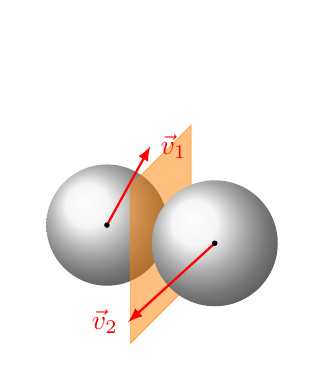
\begin{tikzpicture}
\draw[white] (-1,-1.75) rectangle(2.5,2.5);
  \shade[ball color=gray!10!] (0,0) coordinate(A) circle (0.77) ;
  \draw[orange,fill=orange, opacity=0.5] (0.8,-1,1.3) -- ++(0,2,0) -- ++(0,0,-2) -- ++(0,-2,0) -- cycle;
  \shade[ball color=gray!10!] (1.6,0,0.6) coordinate(B) circle (0.8) ;
  \draw[thick,-latex,red] (A) --+ (0.55,1) node[right]{$\vec v_1$} ;
  \draw[thick,-latex,red] (B) --+ (-1.1,-1) node[left]{$\vec v_2$} ;
%  \draw (4,.2) node[right]{H$^-$} ;
  \foreach \point in {A,B}
  	\fill [black] (\point) circle (1pt) ;
\end{tikzpicture} \hfill
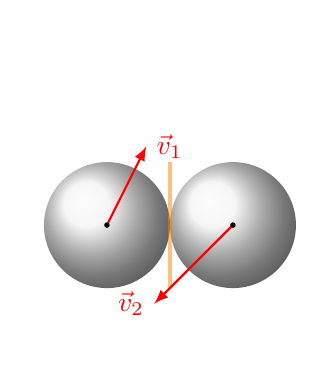
\begin{tikzpicture}
\draw[white] (-1,-1.75) rectangle(2.5,2.5);


  \shade[ball color=gray!10!] (0,0) coordinate(A) circle (0.8) ;
  \shade[ball color=gray!10!] (1.6,0) coordinate(B) circle (0.8) ;
  \draw[very thick, orange, opacity=0.5](0.8,-0.8) --+(0,1.6);
  \draw[thick,-latex,red] (A) --+ (0.5,1) node[right]{$\vec v_1$} ;
  \draw[thick,-latex,red] (B) --+ (-1,-1) node[left]{$\vec v_2$} ;
%  \draw (4,.2) node[right]{H$^-$} ;
  \foreach \point in {A,B}
  	\fill [black] (\point) circle (1pt) ;
\end{tikzpicture} \hfill
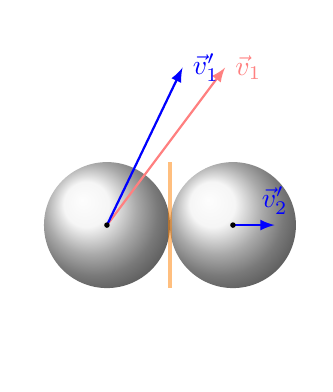
\begin{tikzpicture}
\draw[white] (-1,-1.75) rectangle(2.5,2.5);
  \shade[ball color=gray!10!] (0,0) coordinate(A) circle (0.8) ;
  \shade[ball color=gray!10!] (1.6,0) coordinate(B) circle (0.8) ;
    \draw[very thick, orange, opacity=0.5](0.8,-0.8) --+(0,1.6);
  \draw[thick,-latex,red!50!] (A) --+ (1.5,2) node[right]{$\vec v_1$} ;
  \draw[thick,-latex,blue] (A) --+ (0.96,2) node[right]{$\vec v_1'$} ;
  \draw[thick,-latex,blue] (B) --+ (0.53,0) node[above]{$\vec v_2'$} ;
%  \draw (4,.2) node[right]{H$^-$} ;
  \foreach \point in {A,B}
  	\fill [black] (\point) circle (1pt) ;
\end{tikzpicture} \hfill
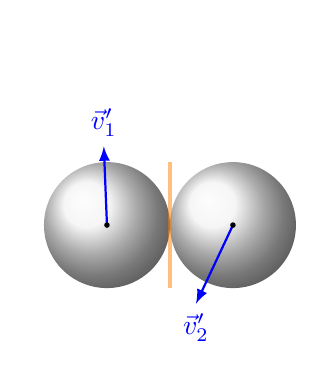
\begin{tikzpicture}
\draw[white] (-1,-1.75) rectangle(2.5,2.5);
  \shade[ball color=gray!10!] (0,0) coordinate(A) circle (0.8) ;
  \shade[ball color=gray!10!] (1.6,0) coordinate(B) circle (0.8) ;
    \draw[very thick, orange, opacity=0.5](0.8,-0.8) --+(0,1.6);
  \draw[thick,-latex,blue] (A) --+ (-0.04,1) node[above]{$\vec v_1'$} ;
  \draw[thick,-latex,blue] (B) --+ (-0.47,-1) node[below]{$\vec v_2'$} ;
%  \draw (4,.2) node[right]{H$^-$} ;
  \foreach \point in {A,B}
  	\fill [black] (\point) circle (1pt) ;
\end{tikzpicture}
\caption{Stoß von 2 Kugeln in 3 Dimensionen (ganz links) kann auf 2 dimensionalen Fall reduziert werden (mitte links) bei dem eine Kugel vor dem Stoß ruht (mitte rechts). Geschwindigkeiten vor dem Stoß jeweils in rot, Geschwindigkeiten der Kugeln nach dem Stoß jeweils in blau }
 \label{fig:hkpotential}
\end{figure} 